%\documentclass[11pt, a4paper]{article}
\documentclass[includeheaders]{scrartcl}
\usepackage{scrlayer-scrpage}
\usepackage{hyperref}
\usepackage[utf8]{inputenc}
% Deutsche Silbentrennung
\usepackage[ngermanb]{babel}
% Unterstützung für Farben
\usepackage[dvipsnames]{xcolor}
% Erweiterte Mathematik-Symbole
\usepackage{amsmath,amscd,amssymb}
% Nummerierte Listen
\usepackage{enumerate}
% Erweiterte Bildeinbettungsoptionen
\usepackage{graphicx}
% Typografisch hochwertige Tabellen
%\usepackage{tabularx,ragged2e,booktabs}
\usepackage{tabularx}
% Unterstützung für Unter-Abbildungen (z.B. 2x2-Matrix)
\usepackage{float}
\usepackage{caption}
\usepackage{subcaption}
% Seitenränder
\usepackage{geometry}
\geometry{a4paper,
	left=2.5cm,
	right=2.5cm,
	top=2.5cm,
	bottom=2.5cm}

% Unterstützung für °-Zeichen
\usepackage{textcomp}
\usepackage{gensymb}
% Formatierung von \paragraph und \subparagraph anpassen
\makeatletter
\renewcommand\paragraph{\@startsection{paragraph}{4}{\z@}%
	{-3.25ex\@plus -1ex \@minus -.2ex}%
	{1.5ex \@plus .2ex}%
	{\raggedsection\normalfont\sectfont\size@paragraph}%
}
\renewcommand\subparagraph{\@startsection{subparagraph}{5}{\z@}%
	{-3.25ex\@plus -1ex \@minus -.2ex}%
	{1.5ex \@plus .2ex}%
	{\raggedsection\normalfont\sectfont\size@subparagraph\mdseries}%
}
\makeatother
\usepackage{lastpage}
\setkomafont{pageheadfoot}{\sffamily} 
\sloppy
\parindent0mm
\parskip3mm

\begin{document}
	
	% o - outer, i - inner, c - center -> location of header/footer-element
%\ohead{
\includegraphics[scale=0.5]{img/HPI-Logo.png}}
%\ifoot{
\includegraphics[scale=0.5]{img/HPI-Logo.png} }
\ifoot{
\includegraphics[scale=0.07]{img/logo}}
\cfoot{Template zur Veranstaltung Modellierung II, \\ Holger Giese, Sommersemester 2016}
\ofoot{\thepage}


	
	\newpage
	
	\title{Entwurfsdokument\\ \small{(Veranstaltung Modellierung II, SoSe 2016)}}
	\date{}
	\author{}
	
	\maketitle
	\begin{table}[H]
		\centering
		\begin{tabular}{lp{7.5cm}}
			\textbf{Projekt:} & Roboterbasiertes Personentransportsystem\\
			&\\
			\textbf{Auftraggeber: }& Prof. Holger Giese \newline Hasso-Platter-Institut \newline Prof.-Dr.-Helmert-Str. 2–3 \newline 14482 Potsdam\\
			&\\
			\textbf{Auftragnehmer: }& Modellierung II – Projektgruppe 5 \\
		\end{tabular}
	\end{table}
	
	
	
	\newpage
	
	\begin{table}[H]
		\centering
		\begin{tabularx}{\textwidth}{|p{4cm}|X|p{4cm}|}
			\hline
			Verantwortlichkeit & Name, Vorname & Datum \\ \hline
			Ansprechpartner    & Bischoff, Sebastian & 17.06.2016 \\
			Bearbeitender      & Sauder, Jonathan & 17.06.2016 \\ 
			Bearbeitender      & Lüpke, Fabian & 17.06.2016 \\ 
			Bearbeitender      & Hering, Jonas & 17.06.2016 \\
			Bearbeitender      & Braun, Jakob & 17.06.2016  \\
			Bearbeitender      & Cremerius, Jonas & 17.06.2016 \\
			Bearbeitender      & Wischner, Jakob & 17.06.2016 \\
			Bearbeitender      & Schwenkert, Daniel & 17.06.2016 \\
			Bearbeitender      & Jäkel, Dominik & 17.06.2016 \\
			Bearbeitender      & König, Bastian & 17.06.2016 \\ \hline
		\end{tabularx}
	\end{table}
	
	\newpage
	
	\tableofcontents

\newpage
\section{Abstrakte Architektur}
In diesem Dokument soll ein Transportsystem mit autonom agierenden Transportvehikeln (\emph{Robots})
entwickelt werden, welche Notfalltransporte für ein Krankenhaus (\emph{Hospital}) erledigen. Die \emph{Robots} werden zu
einem vom \emph{Hospital} angegebenen Ort geschickt, um dort einen Patienten (\emph{Patient}) abzuholen und
danach zur Klinik zu fahren.

Dieser Entwurf basiert auf der in der Analyse erarbeiteten Spezifikation des Systems. Abbildung \ref{KomponentendiagrammAbstrakt} zeigt das abstrakte Komponentendiagramm.

\begin{figure}[H]
	\centering
	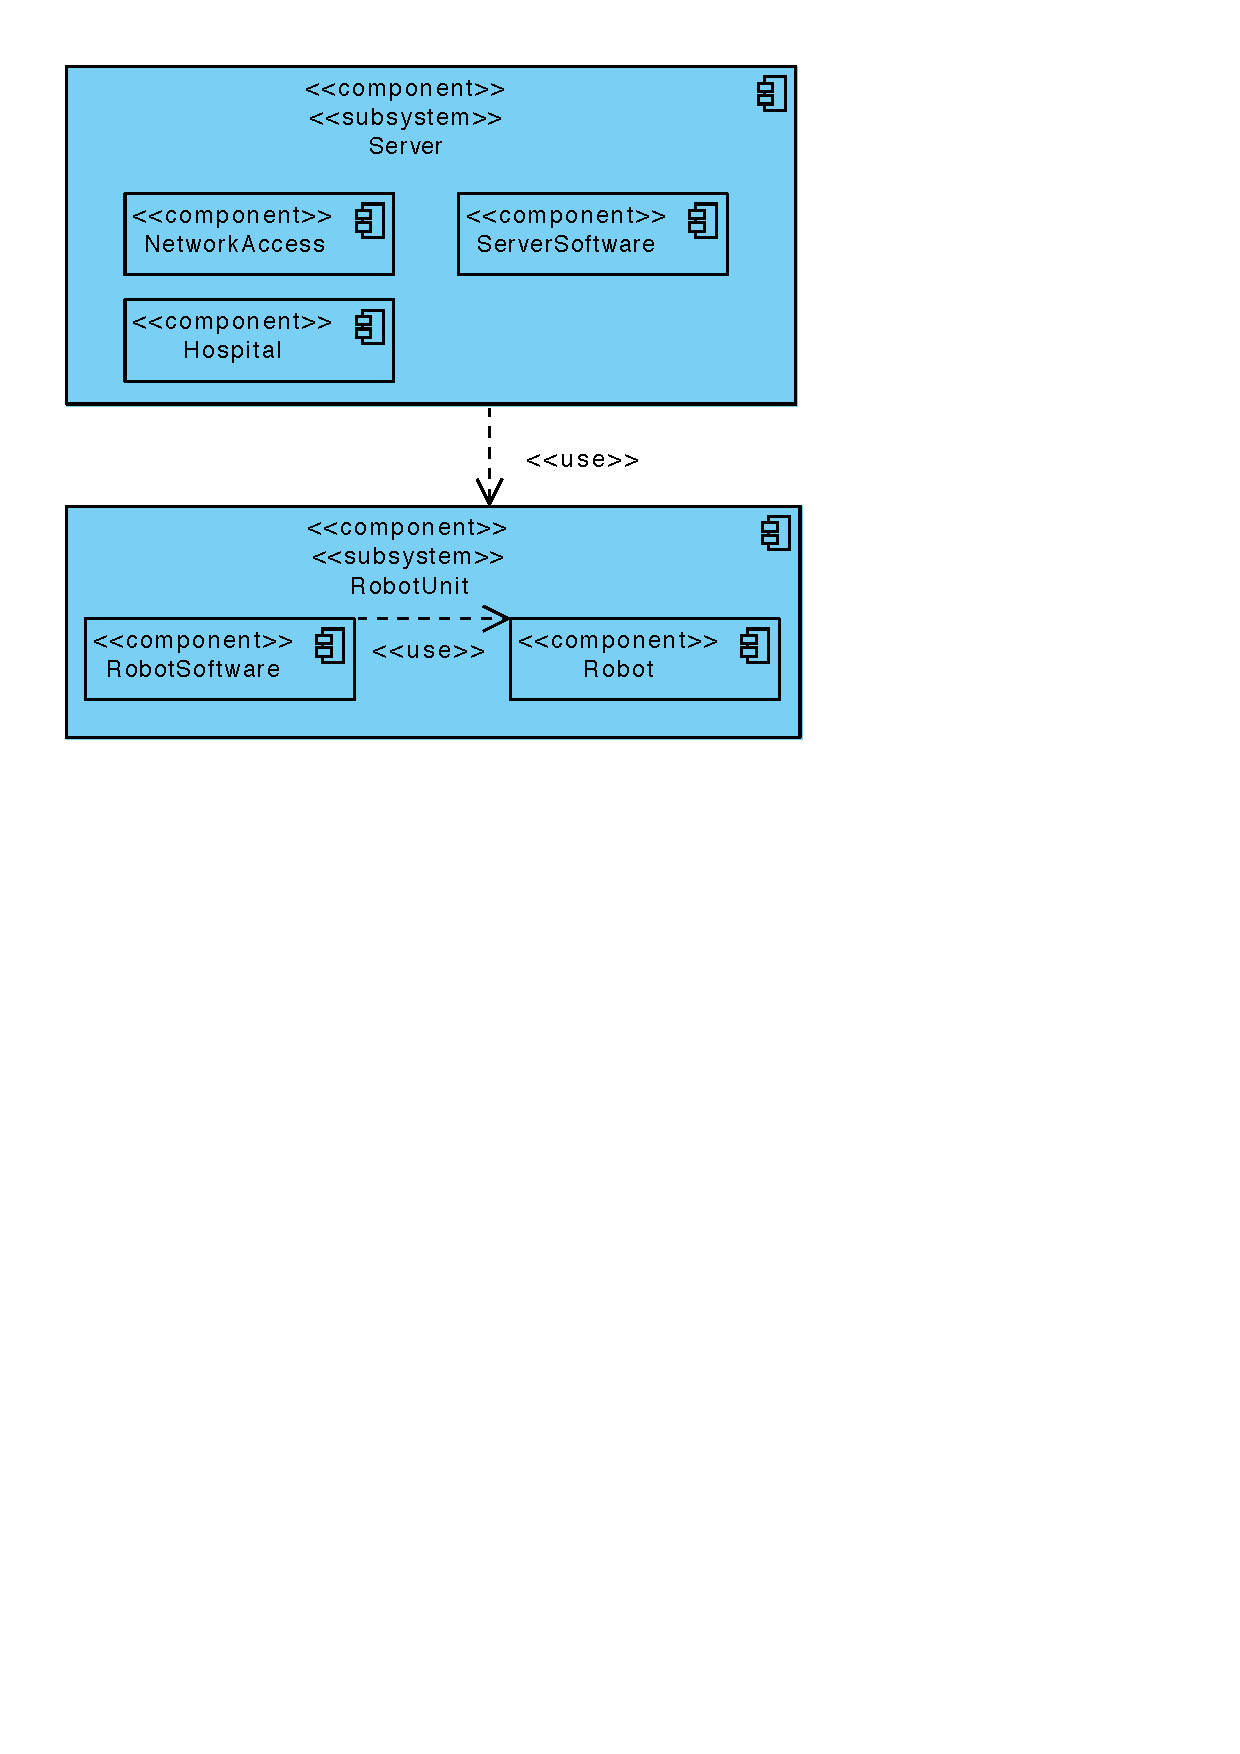
\includegraphics[width=0.6\textwidth]{img/AbstrakteArchitektur}
	\caption{Abstraktes Komponentendiagramm}
	\label{KomponentendiagrammAbstrakt}
\end{figure}

Da eine Komponente mit dem Namen \emph{Robot} bereits vorhanden ist, nennen wir die \emph{Robot}-Hauptkomponente \emph{RobotUnit}. Dieser Name verdeutlicht, dass jeder physische Roboter im System durch diese Hauptkomponente repr\"{a}sentiert wird.


In diesem Kapitel wird die im Rahmen der Analyse ermittelte Einteilung des Systems in Komponenten strukturiert dargestellt. Hierbei soll auch die Interaktion der Komponenten untereinander verdeutlicht werden.

\subsection{Server}

Der \emph{Server} verwaltet die \emph{Tasks} f\"{u}r die \emph{RobotUnits} und beh\"{a}lt \"{U}berblick \"{u}ber die Positionen der \emph{RobotUnits}. Er ist außerdem f\"{u}r die effiziente Allokation der Auftr\"{a}ge an \emph{RobotUnits} zust\"{a}ndig.

\subsubsection{NetworkAccess}

Die Komponente \emph{NetworkAccess} dient der Kommunikation mit dem Netzwerk.

\subsubsection{Hospital}

Die Komponente \emph{Hospital} dient der Kommunikation mit dem Krankenhaus.

\subsubsection{ServerSoftware}

Die Komponente \emph{ServerSoftware} ist die Verwaltungslogik des \emph{Servers}. Sie greift auf die serverseitigen Subsysteme zu und stellt die zentrale Anlaufstelle f\"{u}r alle \emph{RobotUnits} dar.

Bei einer Anfrage ermittelt sie die passende \emph{RobotUnit} und sendet ihr die Position des Ziels.

\subsection{RobotUnit}

Die Komponente \emph{RobotUnit} sublimiert die \emph{RobotSoftware} und \emph{-Hardware} (Komponente \emph{Robot}) als eine Oberkomponente. Sie vereint alle Hard- und Softwareinterfaces dieser Komponenten und leitet die ein- und ausgehenden Nachrichten der \emph{RobotSoftware} an den \emph{Server} weiter. Sie dient somit als \"{u}bergeordnete Schnittstelle f\"{u}r die Kommunikation.

\subsubsection{RobotSoftware}

Die \emph{RobotSoftware} steuert den \emph{Robot} an und verwertet seine Sensordaten. Dazu geh\"{o}rt unter anderem die Fahrlogik und die Verwaltung der \emph{Battery}, damit angenommene \emph{Tasks} auch komplett ausgef\"{u}hrt werden k\"{o}nnen und die \emph{RobotUnit} rechtzeitig die \emph{ChargingStation} erreicht.

\subsubsection{Robot}

Die Komponente \emph{Robot} steht f\"{u}r alle hardwaretechnischen Spezifikationen des \emph{Robots}. Dazu geh\"{o}ren die Fahreinheit und die interne Sensorik sowie die \emph{Battery}.

\newpage
\section{Interaktion der Komponenten}
Auf Basis der Use Cases aus der Analyse wird in diesem Kapitel die Interaktion der einzelnen Komponenten aus Kapitel 1 betrachtet. 
Dabei liegt der Fokus vor allem auf der Interaktion zwischen der RobotUnit und dem Server, wie dessen Austausch mit dem Hospital und der Taxiapp. 
Die Abläufe innerhalb der Komponenten werden dann in Kapitel 8 näher spezifiziert. \\


\subsection*{Interaktion bei Ausführung von \emph{Receive Order \& Cancel Order}}

Elementar ist in diesem Fall der Use Case \texttt{Receive Order} (Use Case 1.1), der es Usern ermöglicht Anfragen oder Notrufe abzusetzen, um ein Taxi oder einen Krankentransporter anzufordern. 
Das System arbeitet mit einer Warteliste für Aufträge von Taxikunden. \\
Krankentransporte werden bei der Vergabe von Aufträgen stets priorisiert und es wird ggf. ein laufender \emph{Task} eines Taxikunden unterbrochen, um einen Robot bereitzustellen. \\
Im Falle des ersten Sequenzdiagramms ist dies mit der Verwendung der \emph{TaxiApp} dargestellt, die wiederum die \emph{Order} mit den Destinations an den Server weitergibt.
Danach wird vom Server überprüft, ob überhaupt Taxis verfügbar sind.
Falls keins mehr verfügbar ist, wird die Anzahl der Kunden in der Wartschlange an die App und somit an den User zurückgegeben. \\
Solange der Taxikunde noch nicht in das Taxi gestiegen ist, kann er mit \texttt{Cancel Order} (Use Case 1.2) seine Bestellung aus dem System (der Warteschlange löschen). \\

\begin{figure}[H]
	\centering
	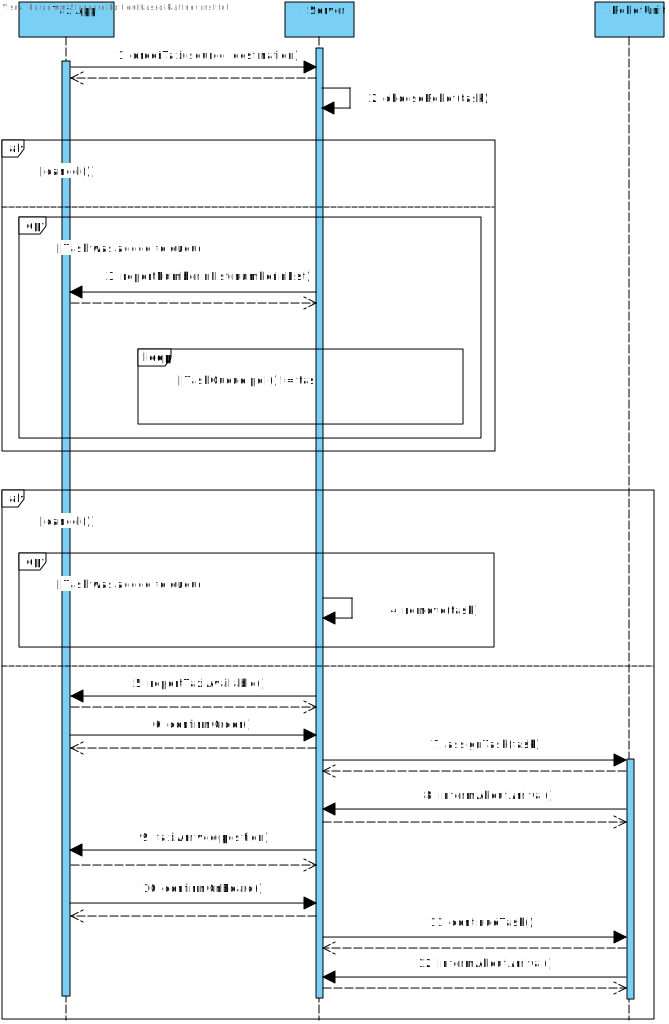
\includegraphics[width=0.9\textwidth]{img/2-Entwurf-ReceiveOrder-Taxi}
	\caption{\emph{ReceiveOrder}-Sequenzdiagramm, falls ein Kunde ein Taxi anfragt}
	\label{SequenzDiagrammInteraktion}
\end{figure}

\begin{figure}[H]
	\centering
	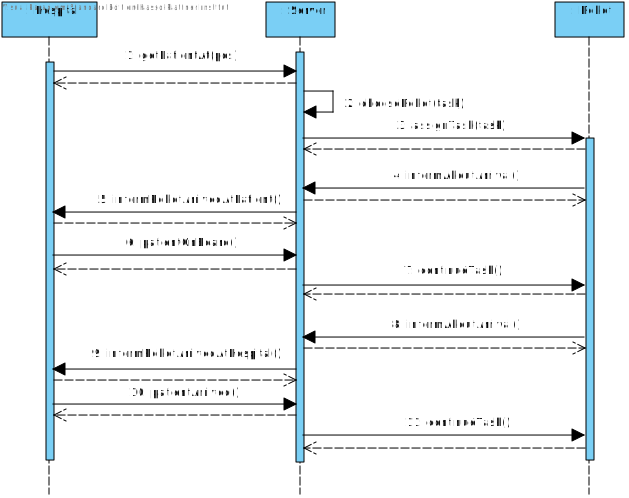
\includegraphics[width=0.9\textwidth]{img/2-Entwurf-ReceiveOrder-Hosp}
	\caption{\emph{RecieveOrder}-Sequenzdiagramm, falls das Hospital einen neuen Patienten meldet}
	\label{SequenzDiagrammInteraktion}
\end{figure}



\subsection*{Interaktion bei Ausführung von \emph{Receive Boarding Confirmation \& Receive Arrival Notification}}

Alle Prozesse laufen wie ersichtlich über den Server, der wiederum die \emph{RobotUnit} fernsteuert. 
So wird für \texttt{Receive Boarding Confirmation} (Use Case 1.3) erst vom Hospital oder der TaxiApp an den Server zurückgemeldet, dass sich der Patient oder der Customer an Bord befindet, bevor die Fahrt aufgenommen werden kann. 
In gleicher Weise wird dem Server mit "Receive Arrival Notification" (Use Case 1.5) zurückgemeldet, dass der Robot wieder für weitere Einsätze verfügbar ist, sobald der Customer den Robot verlassen hat.  \\

\begin{figure}[H]
	\centering
	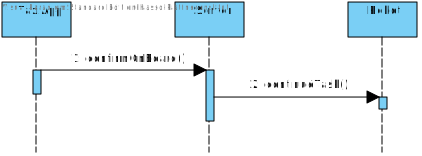
\includegraphics[width=0.9\textwidth]{img/2-Entwurf-ReceiveBoardingConfirmation-taxi}
	\caption{\emph{ReceiveBoardingConfirmation-taxi}-Sequenzdiagramm}
	\label{SequenzDiagrammInteraktion}
\end{figure}

\begin{figure}[H]
	\centering
	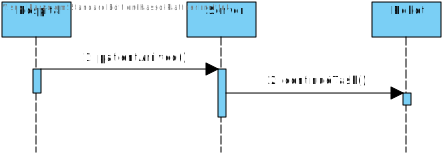
\includegraphics[width=0.9\textwidth]{img/2-Entwurf-ReceiveUnloadConfirmation-hospital}
	\caption{\emph{ReceiveUnloadConfirmation-hospital}-Sequenzdiagramm}
	\label{SequenzDiagrammInteraktion}
\end{figure}


\subsection*{Interaktion bei Ausführung von \emph{Use Cases Perfom Task \& Continue Task}}
Konkret wird der RobotUnit dabei über die Use Cases "Perfom Task" (Use Case 2.2) und "Continue Task" (Use Case 2.3) ein Task zugewiesen, der solange ausgeführt wird, bis der Task abgebrochen wird oder das Ziel erfolgreich erreicht wurde und dies an den Server zurückgemeldet werden kann. \\

\begin{figure}[H]
	\centering
	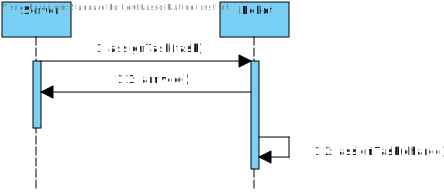
\includegraphics[width=0.9\textwidth]{img/2-Entwurf-PerformTask}
	\caption{\emph{Perform Task}-Sequenzdiagramm}
	\label{SequenzDiagrammInteraktion}
\end{figure}

Die weiteren Use Cases sind diesen untergeordnet; enthalten entweder nur einseitige Server/RobotUnit Kommunikation, wie zum Beispiel bei "Request Repair" (Use Case 1.6) oder haben ihren Fokus vor allem auf den Wechselwirkungen innerhalb der RobotUnit (Siehe dazu Kapitel 8). \\


\newpage
\section{Komponentenschnittstellen}

%3.1 Datentypen
\subsection{\textit{Datentypen}}
Die in Abbildung \ref{KomponentenschnittstellenDiagramm} dargestellten Datentypen werden von den Schnittstellen der eingeführten Komponenten verwendet.

Die Aufgabe des Datentyps SensorData ist es, die Koordination mit dem \emph{Server} zu unterstützen, damit dieser feststellen kann, inwieweit eine Zielposition für einen \emph{Robot} gut zu erreichen ist. Dazu besitzt er als Attribute die Orientierungsrichtung im Koordinatensystem, den Batteriestatus, eine Position im räumlichen Koordinatensystem und zuletzt die mit einem eigenen Datentyp versehene \emph{Destination}. Wird dem \emph{Robot} nun eine neue \emph{Task} zugewiesen, erhält er damit genau diesen Datentyp \emph{Destination}, der die position des Patienten enthält. Mit dem Attribut speed kann der \emph{Server} außerdem genau bestimmen, mit welcher Geschwindigkeit der \emph{Robot} den Patienten anlaufen soll – also die Wichtigkeit des Einsatzes bestimmen.
\vspace{1cm}

	\begin{figure}[H]
		\centering
		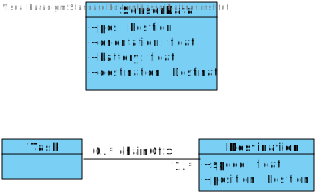
\includegraphics[width=0.6\textwidth]{img/0-Entwurf-3}
		\caption{Datentypen, die in Komponentenschnittstellen verwendet werden}
		\label{KomponentenschnittstellenDiagramm}
	\end{figure}
	\pagebreak

%3.2 Interfaces
\subsection{\textit{Interfaces}}
	%3.2.1 ISensorData
	\subsubsection{\textit{ISensorData}}
	Das Interface \textit{ISensorData} wird vom \textit{Robot} angeboten, um dem Server alle Sensordaten zu senden. Der Server kann anhand dieser jederzeit feststellen, in welchem Zustand sich der \textit{Robot} befindet um diesem dann eine \textit{Task} zuzuweisen.
	\begin{figure}[H]
	\centering
	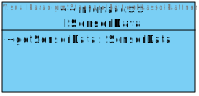
\includegraphics[width=0.4\textwidth]{img/1-Entwurf-3-1_ISensorData}
	\caption{\textit{Interface} ISensorData}
	\label{ISensorData}
	\end{figure}

	%3.2.2 ITask
	\subsubsection{\textit{ITask}}
	Das Interface \textit{ITask} wird vom \textit{Robot} angeboten, um Tasks zu erhalten. Der \emph{Server} kann somit ohne Probleme \textit{Tasks} dem \textit{Robot} zuweisen. Hierbei findet eine unidirektionale Kommunikation zwischen Server und Robot statt.
	\begin{figure}[H]
	\centering
	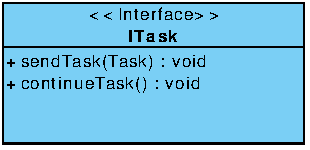
\includegraphics[width=0.4\textwidth]{img/1-Entwurf-3-1_ITask}
	\caption{\textit{Interface} ITask}
	\label{ITask}
	\end{figure}

\newpage
%4
\section{Konkrete Architektur}

\begin{figure}[H]
\centering
\includegraphics[width=0.7\textwidth]{img/4}
\caption{Komponentendiagramm mit den Komponenteninterfaces}
\label{KomponentendiagrammKonkretServer}
\end{figure}

%4.1 Server Software
\subsection{\textit{ServerSoftware}}

Abbildung \ref{KomponentendiagrammKonkretServer} zeigt das konkrete Komponentendiagramm für die Komponente \emph{Server}. Die \emph{ServerSoftware} tätigt in der aktuellen nullten Ausbaustufe direkt Aufrufe an den \textit{Robot},
um den besten \textit{Robot} für eine \textit{Destination} zu ermitteln und einem \textit{Robot} eine \textit{Destination} zuzuweisen.

%4.2 Robot Software
\subsection{\textit{RobotSoftware}}

In Abbildung \ref{KomponentendiagrammKonkretRobot} ist das konkrete Komponentendiagramm der \emph{Robot}-Komponente dargestellt. \emph{RobotSoftware} ist für die Steuerung der \textit{RobotUnit} zuständig. Die von der abstrakten Hardware
des \textit{Robot} angebotenen, vorgegebenen Interfaces \textit{INorthStar, IBattery, IDrive, IDistanceSensors, IBumper} sowie
\textit{IBumperHandler} werden dabei von der \textit{Robot}-Komponente für die konkrete Steuerung der \textit{RobotUnit} genutzt.

\newpage
\section{Komponenten}

%5.1 Server Software
\subsection{Komponente \textit{ServerSoftware}}
\begin{figure}[H]
\centering
\includegraphics[width=0.75\textwidth]{img/Komponenten1.png}
\caption{\textcolor{blue}{Durch eigene Diagramm ersetzen}}
\label{KomponentenStruktur1}
\end{figure}
Die Komponente \textit{ServerSoftware} umfasst 4 Klassen: \textit{TaskSystem}, \textit{Destination}, \textit{RobotControlSystem} und \textit{Virtual Robot}.
Das \textit{TaskSystem} verwaltet die \textit{Tasks}, in der nullten Ausbaustufe fallen dabei allerdings noch nicht viele Aufgaben an, 
da es keine Priorisierungen, unterschiedliche Arten von \textit{Tasks} oder dergleichen gibt. Die Klasse \textit{Destination} ist die Klasse 
der Aufgaben, die vom \textit{TaskSystem} verwaltet werden. Das \textit{RobotControlSystem} verteilt die \textit{Tasks} auf die \textit{Robots}. 
Dabei findet die Auswahl anhand der zurückgegebenen \textit{SensorData} der einzelnen \textit{Robots} statt. Bei \textit{VirtualRobot} handelt 
es sich um eine Kapselung der Kommunikation mit den \textit{Robots}. Hier werden alle von der Komponente \textit{Robot} bereitgestellten 
\textit{Interfaces} implementiert.
%5.1 Robot Software
\subsection{Komponente \textit{RobotSoftware}}
\begin{figure}[H]
\centering
\includegraphics[width=0.85\textwidth]{img/Komponenten2.png}
\caption{\textcolor{blue}{Durch eigene Diagramm ersetzen}}
\label{KomponentenStruktur2}
\end{figure}
Die Komponente \textit{RobotSoftware} enthält 3 Klassen: \textit{DrivingSystem}, \textit{RobotController} und \textit{Destination}. 
Das \textit{DrivingSystem} stellt eine Abstraktion der Hardware dar und wird dazu genutzt, Ziele anzufahren und Dabei, 
falls nötig, Hindernisse zu umfahren. Dazu greift es auf die von der Hardware bereitgestellten \textit{Interfaces} zurück. 
Um auf Kollisionen reagieren zu können, implementiert das \textit{DrivingSystem} die Schnittstelle \textit{IBumperHandler}
Der \textit{RobotController} stellt die Interfaces \textit{ITask} und \textit{ISensordata} (dem Server) zur Verfügung und verwaltet den gerade 
zu absolvierenden \textit{Task}. Zur Messwertübermittlung greift er zum einen auf das \textit{DrivingSystem} und zum anderen auf das 
von der Hardware angebotenen \textit{Interface} \textit{IBattery} zu.


\newpage
\section{Paketstruktur}
Dieser Abschnitt beschreibt die strukturelle Gliederung des Projektes in einem Paketdiagramm, dargestellt in Abbildung \ref{Paketstruktur}.

Die Pakete \textit{RobotSoftware} und \textit{Server} werden getrennt betrachtet, da es eine physikalische Trennung zwischen den Geräten gibt, auf denen die jeweiligen Pakete vorhanden sein müssen.

Im \textit{Common}-Paket sind alle Klassen enthalten, die sowohl vom \textit{Robot}- als auch vom \textit{Server}-Paket genutzt werden. 
So sind die Datentypen \textit{Destination}, \textit{Task} und \emph{SensorData} enthalten. 
Eine Möglichkeit zur Unterscheidung von \textit{Tasks} ist wichtig, da zwischen vom \textit{Server} zugeteilten \textit{Tasks}, insbesondere Taxi- und Krankenhaustransporten, und vom \textit{Robot} selbst zugeteilten Ladestationen als Ziel unterschieden werden muss. 

Das Paket \textit{Robot} enthält das Paket \textit{HardwareInterfaces}, welches die Möglichkeiten schafft, die Hardwareschnittstellen des \textit{Robots} direkt anzusprechen. 
Das Paket \textit{RobotControl} enthält Klassen zur Steuerung und Speicherung des Zustandes des \textit{Robots}, sowie die \emph{Handler}, die den Hardwareschnittstellen übergeben werden.

Der Server hat Klassen zur Verwaltung der \textit{Robots} und ihren zugehörigen \textit{Tasks}. 
Außerdem sind im \textit{Server} Paket auch Klassen zur Kommunikation mit dem \textit{Hospital} und den Taxikunden vorhanden.

\begin{figure}[H]
\centering
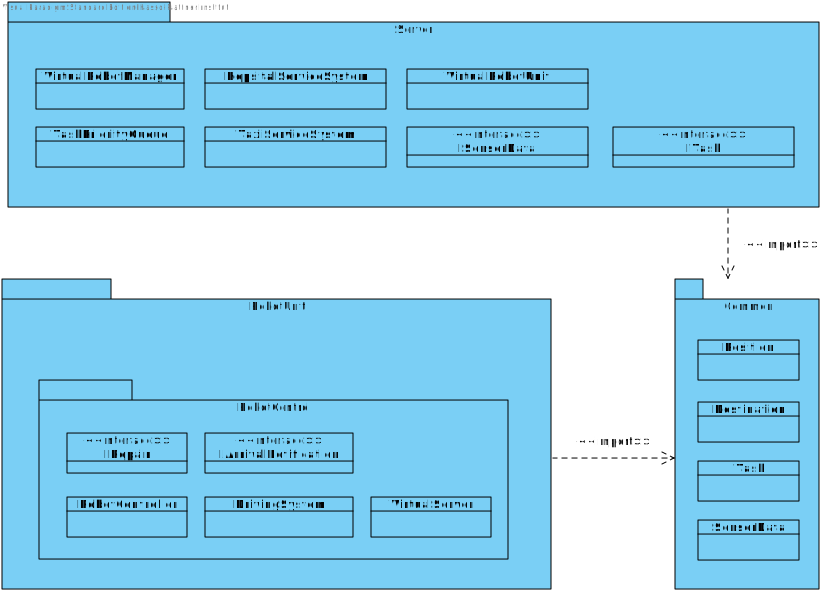
\includegraphics[height=0.8\textwidth, angle=90]{img/6_paketdiagramm}
\caption{Paketdiagramm zur strukturellen Gliederung der Software}
\label{Paketstruktur}
\end{figure}

\newpage
%7
\section{Paketdetails}

%7.1 Paket Robot
\subsection{Paket \textit{Robot}}
	\begin{figure}[H]
	\centering
%	\includegraphics[width=0.6\textwidth]{../images/Paketdetails.png}
	\caption{\textcolor{blue}{HIER KOMMT DAS ROBOT - PAKETDIAGRMAM HIN}}
	\label{Paketdetails}
	\end{figure}
	Im folgenden beschreiben wir die wichtigen Klassen des Pakets \textit{Robot} 
	und ihre zugehörigen wichtigen Methoden, sowie ihre Interaktion zwischeneinander. 


	%7.1.1 RobotController
	\subsubsection{Beschreibung der Klasse \textit{RobotController}}
		\begin{figure}[H]
		\centering
		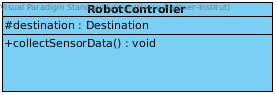
\includegraphics[width=0.6\textwidth]{../images/Iteration0_Entwurf_7-1-1_Klasse_RobotController.png}
		\caption{\textcolor{blue}{Durch eigene Diagramme ersetzen}}
		\label{BeschreibungKlasse1}
		\end{figure}
		
		%#destination : Destination
		
		Die Klasse \textit{RobotController} ist die Hauptklasse des \textit{Robots}, 
		da sie den aktuellen Zustand des \textit{Robots} enthält.
		So hat diese Klasse die Möglichkeit höchstens eine \textit{Destination} zu speichern. 
		Diese \textit{Destination} kann ein vom \textit{Server} zugeteiltes Ziel sein, 
		der dem \textit{Robot} zugehörige \textit{Charger}, oder gerade kein Ziel, 
		also \textit{null} sein. Nur wenn der \textit{Robot} gerade keine \textit{Destination} 
		gespeichert hat, kann er neue Aufträge vom \textit{Server} annehmen.

			%7.1.1.1 #collectSensorData():void
			\subsubsection{Beschreibung der Methode \textit{collectSensorData}}
			Die Methode \textit{collectSensorData} wird von der Methode \textit{recieveMessage} 
			aus der Klasse \textit{RobotCommunication} aufgerufen, wenn eine Neue \textit{Message} 
			vom Server eingegangen ist, welche den \textit{Robot} dazu auffordert, Informationen 
			über seinen Zustand zu senden. Der \textit{Robot} fragt dann seine Hardwareschnittstelle 
			nach seiner Position und seinem Akkustand an, und verfasst eine neue \textit{Message} 
			die diese Informationen, sowie seinen Aktuellen Zustand bzw. seine aktuelle \textit{Destination} enthalten.
			

	%7.1.2 DrivingSystem
		
	\subsubsection{Beschreibung der Klasse \textit{DrivingSystem}}
		\begin{figure}[H]
		\centering
		\includegraphics[width=0.6\textwidth]{../images/Iteration0_Entwurf_7-1-2_Klasse_DrivingSystem.png}
		\caption{\textcolor{blue}{Durch eigene Diagramme ersetzen}}
		\label{BeschreibungKlasse1}
		\end{figure}
		
		%#currentSpeed:float
		Diese Klasse beschreibt den aktuellen Zustand des Fahrsystems des \textit{Robots}. 
		Es sind Informationen über die aktuelle Geschwindigkeit enthalten und die Methode, 
		die gerade ausgeführt wird, gibt Auskunft über die aktuelle Beschäftigung des \textit{Robots}.

			%7.1.2.1 	#driveToDestination(destination: Destination, arrivalHandler: ArrivalHandler): void
			
			\subsubsection{Beschreibung der Methode \textit{driveToDestination}}
			\begin{figure}[H]
			\centering
			\includegraphics[width=0.6\textwidth]{../images/Iteration0_Entwurf_7-1-2-1_Methode_driveToDestination.png}
			\caption{\textcolor{blue}{Durch eigene Diagramme ersetzen}}
			\label{BeschreibungKlasse1}
			\end{figure}

			Wenn diese Methode aufgerufen wird, macht der \textit{Robot} sich auf den Weg zur 
			übergebenen \textit{Destination}. Wenn der \textit{Robot} an dieser \textit{Destination} 
			angekommen ist, wird die Methode des übergebenen \textit{ArrivalHandlers} ausgeführt. 
			Wenn sich ein \textit{Obstacle} auf dem Weg befindet, wird die Methode \textit{driveAroundObstacle} 
			aufgerufen, bis das \textit{Obstacle} umfahren wurde.

			%7.1.2.2    -driveAroundObstacle(destination: Destination): void
			\subsubsection{Beschreibung der Methode \textit{driveAroundObstacle}}
			\begin{figure}[H]
			\centering
			%TODO: Sequenzdiagramm
			\includegraphics[width=0.6\textwidth]{img/BeschreibungKlasse1.png}
			\caption{\textcolor{blue}{Durch eigene Diagramme ersetzen}}
			\label{BeschreibungKlasse1}
			\end{figure}

			Diese Methode wird von \textit{driveToDestination} mit des Position eines \textit{Obstacles} aufgerufen, 
			wenn ein \textit{Obstacle} zu umfahren ist.
			Dabei entscheidet sich der Roboter zunächst ob er links oder rechts an dem \textit{Obstacle} vorbeifährt, 
			und hält sich dann mithilfe seiner Sensoren immer auf einem bestimmten Abstand zum Hindernis, bis zwischen 
			\textit{Obstacle} und der Luftlinie zur \textit{Destination} genug Platz für den \textit{Robot} ist.
	
	%7.1.3 RobotCommunication
	\subsubsection{Beschreibung der Klasse \textit{RobotCommunication}}
		\begin{figure}[H]
		\centering
		\includegraphics[width=0.6\textwidth]{img/BeschreibungKlasse1.png}
		\caption{\textcolor{blue}{Durch eigene Diagramme ersetzen}}
		\label{BeschreibungKlasse1}
		\end{figure}
		%	-communicationID: int
		
			%7.1.3.1	#sendMessage(m: Mesasage): void
			\subsubsection{Beschreibung der Methode \textit{sendMessage}}
	
			%7.1.3.2	#receiveMessage(): void
			\subsubsection{Beschreibung der Methode \textit{receiveMessage}}
	

	\begin{figure}[H]
	\centering
	\includegraphics[width=0.6\textwidth]{img/BeschreibungKlasse2.png}
	\caption{\textcolor{blue}{Durch eigene Diagramme ersetzen}}
	\label{BeschreibungKlasse2}
	\end{figure}

\newpage
\section{Abläufe}

Während in Kapitel 3 die Interaktion der Hauptkomponenten Server und der RobotUnit abgehandelt wurden, werden im Folgenden die Abläufe der Use Cases genauer spezifiziert und auch interne Komponentenabläufe beschrieben, im Speziellen die Abläufe innerhalb der RobotUnit.

\subsection*{Use Cases in Wechselwirkung mit der IDrive Komponente }
Sobald der Roboter mit Perform Task(Usecase 2.2)  und Continue Task( Use Case  2.3) eingehende Aufgaben erhält, wird in jedem Fall das Ziel für die IDrive-Komponente spezifiziert. Und der Roboter setzt, sofern kein Abbruchanweisung dazwischenspielt, seinen Weg ungebrochen fort. Hat die IDrive-Komponente im Wechselspiel mit der INorthStar-Komponente für die räumliche Orientierung dann ihren Zielort erreicht, wird dies wiederum an die RobotUnit übermittelt, die weiter mit dem Server über ihre IWlanAdapter Komponene kommunzieren kann, wie es im UseCase ReceiveArrivalNotification( Use Case 1.5) der Fall ist.
\\

		\begin{figure}[H]
		\centering
		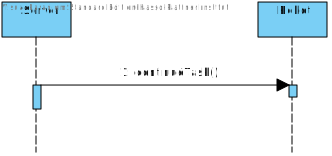
\includegraphics[width=1\textwidth]{img/2-Entwurf-ContinueTask.svg}
		\caption{Sequenzdiagramm von \emph{Read Sensors}}
		\label{ReadSensors}
	\end{figure}
	
	\begin{figure}[H]
		\centering
		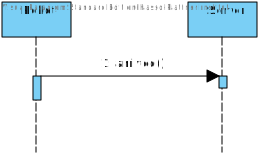
\includegraphics[width=1\textwidth]{img/2-Entwurf-ReceiveArrivalNotification.svg}
		\caption{Sequenzdiagramm von \emph{Read Sensors}}
		\label{ReadSensors}
	\end{figure}

	\subsection*{Interaktion bei Ausführung von Use Case 2.1 – \emph{Read Sensors}}
In der folgenden Grafik wird der reine Informationsanfrageprozess zwischen Server und der RobotUnit dargestellt, auf dessen Basis ersterer alle notwendigen Daten über die zur Verfügung stehenden RobutUnits jederzeit abrufen kann; insbesondere wenn eine optimale Auswahl für ein Taxi oder einen Krankentransporter getroffen werden soll. Nach der Anfrage, wird die RobotUnit alle nötigen Informationen nacheinander abfragen: Sowohl die Position als auch die Orientierungsrichtung werden von der INorthStar-Komponente zurückgeliefert. Für den Batteriestatus muss die IBattery-Komponente angefragt werden. Erst wenn alle Informationen als Gesamtpaket bereitstehen, können sie an den Server zurückgemeldet werden.

\\

	\begin{figure}[H]
		\centering
		\includegraphics[width=1\textwidth]{img/0-Entwurf-8-ReadSens}
		\caption{Sequenzdiagramm von \emph{Read Sensors}}
		\label{ReadSensors}
	\end{figure}

	
	\subsection*{Interner Ablauf im Falle der Begegnung eines Hindernisses}}
	Sowohl die Methoden Path Around Obstacle als auch der Use Case Drive AroundObstacle sind beides Bestandteile des internen Ablauflaufprozesses, der im Falle eines auftauchenden Hindernisses einsetzt. Die RobotUnit befindet sich dabei stets in einem Fahrvorgang, der stets konkret mit der Zielposition und er Geschwindigkeit vom Server eingestellt wurde. So reagiert intern seine Software mit dem IDistanceSensor, wenn ein Hindernis um ihn herum auftaucht und dieses mit Hilfe der durch die Sensoren gesammelten Informationen umfahren werden muss. Dabei muss der Roboter ausdrücklich zwischen einem Roboter und einem unbeweglichen Hindernis unterscheiden, um so vorherzubestimmen wie eine optimale Ausweichbewegung aussehen wird. Auch wenn die IDistanceSensor die vollständige Umgebung um den Roboter wahrnehmen kann, bezieht sich dies jedoch primär auf vor dem Roboter liegende Hindernisse. Dieser Prozess ist Bestandteil des Methode Choose Path around Obstacle und geht dann in den Methode Drive Around Obstacle über. Der Roboter koordiniert sich dort mit seiner IDrive-Komponente und seinen Sensoren, um langsam an einem unbeweglichen Objekt vorbeizufahren. Dabei fährt er immer eine kleine Distanz parallel zur Kante des Obstacles und prüft ob der Weg zur Destination wieder frei ist. Ist dies der Fall nimmt er den Fahrtprozess wieder auf. Erkennen sich zwei Roboter hingegen gegenseitig als Hindernis weichen beide mit Hilfe ihrer IDrive Komponente nach rechts aus, und nehmen anschließend den normalen Fahrbetrieb wieder auf. Sollten all diese Vorkehrungen dennoch nicht helfen, setzt der IBumperHandler ein. Dieser kann sofortig über den Server Request Repair( Use Case 1.6) anfordern oder im Falle das Passagiere an der Kollision beteiligt waren, einen Krankentransporter anrufen.
 \\
	
	\begin{figure}[H]
		\centering
		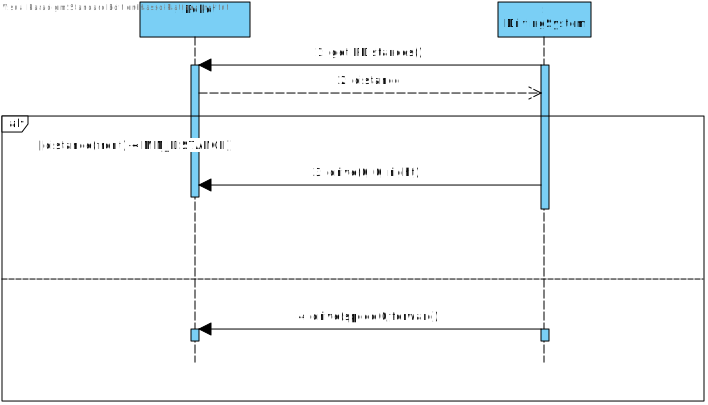
\includegraphics[width=0.95\textwidth]{img/1-Entwurf-8-DriveArroundObstacle}
		\caption{Sequenzdiagramm von \emph{Drive arround Obstacle}}
		\label{UmfahrenvonstatichenObjekten}
	\end{figure}
	\vspace{1cm}
	
	\subsection*{Interner Ablauf Charging}
	Charging ist ein spezieller interner Ablauf der RobotUnit für den keine weitere Kommunikation mit der Komponente Server stattfinden muss, dafür allerdings zwischen der RobotUnit und der ChargingStation. Hat der Roboter einen bestimmten kritischen Ladestand erreicht (, den er regelmäßig überprüft), läuft er die ChargingStation-Komponente an. Der Ladevorgang triggert automatische, sobald der Roboter die Position der Ladestation erreicht hat, und interagiert solange mit ihr bis seine Batterie wieder aufgeladen ist. Innerhalb des Robots werden zum Anfahren der ChargingStation die Komponenten IBatterie mit der Position der Robotereigenen Ladestation und IDrive benötigt. Konkret: Wenn IDrive arrived() zurückgibt, kann der Ladevorgang begonnen werden.
	\vspace{1cm}
	
	\begin{figure}[H]
		\centering
		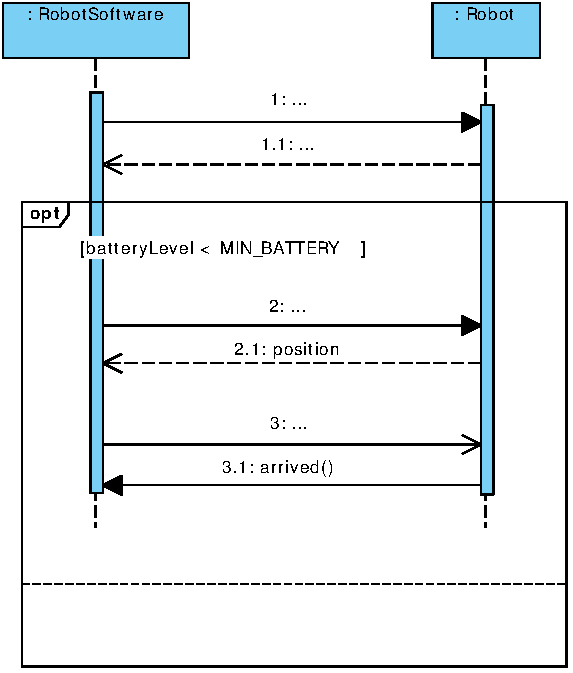
\includegraphics[width=0.65\textwidth]{img/0-Entwurf-8-Charging}
		\caption{Sequenzdiagramm von \textit{Charging}}
		\label{Charging}
	\end{figure}

\newpage
\section{Produkteinsatz}

In diesem Abschnitt wird der geplante Einsatz des Systems beschrieben, wobei
insbesondere auf die Systemumgebung, in der das Produkt eingesetzt werden soll,
und die Zuordnung der Software zu dieser eingegangen wird.
Abbildung \ref{ProdukteinsatzKomp}
zeigt ein Verteilungsdiagramm des Gesamtsystems, dessen Komponenten im Folgenden
erläutert werden.

Das Gesamtsystem besteht im Wesentlichen aus einem \emph{Server}, der mit mindestens einer
\emph{Robot Unit} verbunden ist. Zwischen \emph{Server} und \emph{Robot Units} kann über
einen auf beiden Seiten verfügbaren \emph{Wlan\-Adapter} über ein
Funknetzwerk kommuniziert werden.

Auf dem \emph{Server} und den \emph{Robot Units} läuft ein \emph{Java Runtime Environment},
das dem Ausführen der entsprechenden Software dient.

\emph{RobotUnit.jar} dient der Kapselung aller verfügbaren Funktionen. Es bietet Zugriff
auf \emph{RobotSoftware} und \emph{Robot}.

\emph{Server.jar} agiert analog zu \emph{RobotUnit.jar} und bietet Zugriff auf alle grundlegenden 
Funktionalitäten von \emph{ServerSoftware}, \emph{Hospital} und \emph{TaxiApp}.

Zusätzlich benötigte Funktionalitäten werden aus dem \emph{Common}-Paket importiert und sind
sowohl bei den \emph{Robot Units} als auch dem \emph{Server} verfügbar.

\begin{figure}[H]
	\centering
	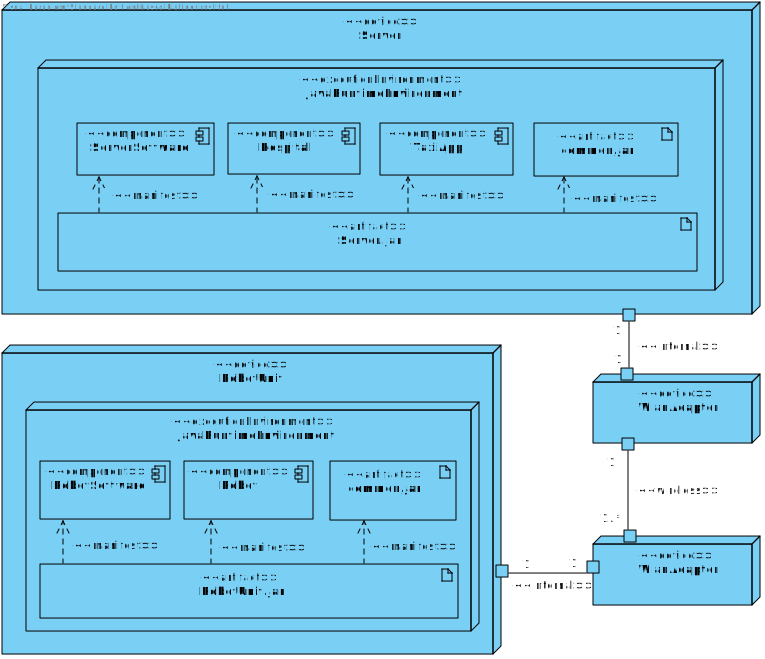
\includegraphics[width=1\textwidth]{img/2-Entwurf-9-Produkteinsatz}
	\caption{Verteilungsdiagramm des Gesamtsystems}
	\label{ProdukteinsatzKomp}
\end{figure}


\end{document}
